\documentclass{article}
\usepackage[utf8]{inputenc}
\usepackage{listings}
\usepackage{amsmath,amssymb}
\usepackage{graphicx}
\usepackage{xcolor}

\usepackage{inconsolata}
\lstset{
  basicstyle=\ttfamily,
}

\usepackage{hyperref}
\hypersetup{
    colorlinks,
    citecolor=black,
    filecolor=black,
    linkcolor=black,
    urlcolor=black
}


\renewcommand{\baselinestretch}{1.2}

\setlength{\parskip}{1em}
\definecolor{codegreen}{rgb}{0,0.6,0}
\definecolor{codegray}{rgb}{0.5,0.5,0.5}
\definecolor{codepurple}{rgb}{0.58,0,0.82}
\definecolor{backcolour}{rgb}{0.95,0.95,0.92}

\lstdefinestyle{mystyle}{
    backgroundcolor=\color{backcolour},   
    commentstyle=\color{codegreen},
    keywordstyle=\color{magenta},
    numberstyle=\tiny\color{codegray},
    basicstyle=\ttfamily\footnotesize,
    breakatwhitespace=false,         
    breaklines=true,                 
    captionpos=b,                    
    keepspaces=true,                 
    numbers=left,                    
    numbersep=5pt,                  
    showspaces=false,                
    showstringspaces=false,
    showtabs=false,                  
    tabsize=2
}

\lstset{style=mystyle}


\title{	\ Trabajo Práctico Nro 1: Algoritmos Greedy y Dividisión y conquista}


\author{    Nestor Huallpa, \textit{Padrón Nro. 88614}\\
            \texttt{ huallpa.nestor@gmail.com }\\\\  
            Pepe, Jonathan Leonel, \textit{Padrón Nro. 94692}\\
            \texttt{ jonathan.leonel.pepe@gmail.com }\\\\     
            Ignacio Argel, \textit{Padrón Nro. 104351}\\
            \texttt{ iargel@fi.uba.ar }\\\\      
            Mateo Javier Ausqui, \textit{Padrón Nro. 102593}\\
            \texttt{ mausqui@fi.uba.ar }\\\\              
            \texttt{\footnotesize 1º Entrega: 20/05/2020}\\
            \textbf{Grupo: En cuarentena}
            \\\\\\\\\\\\\\\\\\
            \normalsize{1do. Cuatrimestre de 2020}\\ 
            \normalsize{75.29/95.06 Teoría de Algoritmos I} \\
            \normalsize{Facultad de Ingeniería, Universidad de Buenos Aires} \\}


\date{}

\begin{document}

\maketitle
% quita el número en la primer página
\thispagestyle{empty}

\newpage{}
\tableofcontents

% quita el número en la primer página
\thispagestyle{empty}

\newpage{}

\newpage
\section{Introducción}

En el presente trabajo plantearemos dos soluciónes mediante algoritmos para al problema de ausentismo de una empresa y sobre una nueva regulación industrial. 

\section{Un problema de ausentismo}

\subsection{Descripción del problema}

Una empresa de tercerización laboral nos convoca para que le ayudemos con un problema de ausentismo laboral. 
Tiene un conjunto de \(n\) empleados que realizan tareas en diferentes puntos de la ciudad. 
El turno de cada empleado \(i\) comienza en \(T_i(i)\) y termina en \(T_f(i)\) y durante todo ese lapso tiene que estar en la ubicación establecida. 
La dirección de la empresa sospecha que algunos de sus empleados suelen faltar sin aviso. Para verificarlo contrataron a la empresa “Dystopian Technologies Inc.” (DTI). 
Esta empresa implanta un microchip con un código único en cada empleado. Mediante rastreo satelital pueden conocer dónde se encuentra cada chip implantado en cualquier momento. Además posee el cronograma completo de las tareas.

DTI brinda un sistema que mediante una consulta (encendido / apagado) nos devolverá cuáles empleados aún no controlados y en horario de trabajo se encuentran en su sitio y cuáles no.
\subsection{Hipótesis}
\begin{itemize}
    \item Los tiempos informados son enteros de 0 en adelante.
    \item DTI les cobra por cada encendido / apagado.
    \item Cada encendido / apagado es casi instantáneo y se lo programa para algún valor de t entero.
    \item Cada encendido / apagado (y su consecuente rastreo) es \(O(1)\).
    \item El empleado una vez en su puesto no se retira hasta concluir su turno.
\end{itemize}

\subsection{Descripción del algoritmo}

Tenemos un conjunto de empleados \(\{1,2,..,n\}\); el empleado \(i^{th}\) corresponde a un intervalo de tiempo que comienza al instante \(s(i)\) y finaliza de trabajar al instante \(f(i)\).
Diremos que un subconjutno de empleados es compatible si no hay dos de ellos que al mismo tiempo se superpongan y nuestro objetivo es encontrar un subconjunto compatible tan grande como sea posible.
El tiempo \(f(i)\) de los empleados del conjunto seran los tiempos que deben encender el sensor de DTI.

La idea basica para el algoritmo greedy es seleccionar el primer empleado \(i_1\), una vez seleccionado, descartamos del resto de los empleados a aquellos que tienen una intersección con el seleccionado \(i_1\).
Luego seleccionamos el empleado \(i_2\) y volvemos a descartar todos los empleados que intesecan con el empleado \(i_2\). Continuamos de esta manera hasta que nos quedamos sin empleados para evaluar.  

De esta forma nos iremos quedando con los empleados que terminan primero, o sea el empleado que tenga menor \(f(i)\) para poder tomar el valor del instante \(f(i)\) como el tiempo donde se debe encender el sensor para 
abarcar la mayor cantidad de empleados por cada encendido del sensor. El resultado sera \textbf{óptimo} si obtenemos abarcamos a todos los empleados con la menor cantidad de encendidos del sensor de DTI. Para esta solución nos basamos en el problema de planificación de intervalos.

El algoritmo funciona de la siguiente manera:
\begin{enumerate}
    \item Ordena la lista de empleados de menor a mayor según el valor \(t_f\).
    \item Selecciona el \(t_f\) del primer empleado de la lista de empleados y guarda el valor en \(t_{fx}\).
    \item Añade \(t_{fx}\) a la lista de tiempos de encendido (la cual indicará en qué momentos debe encenderse el módulo DTI).
    \item Verifica si el \(t_i\) del próximo empleado en la lista es mayor a \(t_{fx}\), si lo es guarda en \(t_{fx}\) el \(t_f\) de dicho empleado y añade \(t_{fx}\) a la lista de tiempos de encendido.
    \item Repite el paso 4 hasta hasta terminar de recorrer la lista de empleados.
    \item Los tiempos guardados en la lista de tiempos de encendido son los tiempos en los cuales debe encenderse el módulo DTI.
    
\end{enumerate}


\subsection{Pseudocódigo del algoritmo}

\begin{lstlisting}[language=Python, caption=Algoritmo de greddy para tiempos de encendido]
lista[int] obtenerTiemposDeEncendido(lista[empleado] listaEmpleados)

	OrdenarDeMenorAMayorPorTiempoFinal(listaEmpleados)

	tiempoFin = listaEmpleados(0).obtenerTF

    listaTiemposEncendidos.agregar(tiempoFin)

	i = 1

	Mientras(listaEmpleados != fin)

		Si(listaEmpleados(i).obtenerTI > tiempoFin)

			tiempoFin = listaEmpleados(i).obtenerTF

	        listaTiemposEncendidos.agregar(tiempoFin)

		i++

Devolver listaTiemposEncendidos	
\end{lstlisting}    


Adicionalmente, creamos la función ConsultarDTI que recibe una lista con los tiempos en los cuales debe encenderse dicho módulo. 
Esta función espera hasta que la hora del sistema sea igual a los tiempos de encendido que se encuentran en el listado. 
Cuando esto sucede se enciende el módulo DTI (método EncenderDTI) y se imprime por pantalla la lista de empleados que este 
método devuelve (aquellos que se encuentran en sus puestos de trabajo). 

Cabe aclarar que listaTiemposEncendidos se encuentra ordenada de menor a mayor, 
por la manera en que fue construida en el método obtenerTiemposDeEncendido, y que DTI se encenderá tantas veces durante el transcurso del día como tiempos haya en este listado.

\begin{lstlisting}[language=Python, caption=Proceso de consulta a DTI]

void ConsultarDTI(lista[int] listaTiemposEncendidos)

    i = 0
        
    Mientras listaTiemposEncendidos != fin

        Esperar hasta que HoraSistema() == listaTiemposEncendidos(i)

        Imprimir(EncenderDTI())
        
        i++

\end{lstlisting}    


\subsection{Ejemplo de ejecución}

Solo se detallan los \(t_i\) y \(t_f\) de cada empleado. 
Se marcan en color rojo los empleados que se recorren y en verde el empleado del cual 
se consulta su tf (color azul) para guardar en la lista que contendrá los tiempos en los 
cuales debe encenderse DTI.


\underline{Preparación} (ordenar de menor a mayo según tf):

listaEmpleados = \{(1,4) - (2,4) - (2,5) - (3,5) - (3,6) - (1,6) - (2,7) - (5,8) - (2,8) - (6,8) - (1,10) - (5,10) - (7,10) - (7,11) - (8,11) - (10,12) - (11,12) - (12,14)\}

listaTiemposEncendidos = \{\}


\underline{Primera ejecución del bucle:}

listaTiemposEncendidos = \{\textcolor{blue}{4}\}

listaEmpleados = \{ \textcolor{green}{(1,4)} - \textcolor{red}{(2,4) - (2,5) - (3,5) - (3,6) - (1,6) - (2,7)} - (5,8) - (2,8) - (6,8) - (1,10) - (5,10) - (7,10) - (7,11) - (8,11) - (10,12) - (11,12) - (12,14)\}

\underline{Segunda ejecución del bucle:}

listaTiemposEncendidos = \{4 - \textcolor{blue}{8}\}

listaEmpleados = \{ \textcolor{green}{(1,4)} - \textcolor{red}{(2,4) - (2,5) - (3,5) - (3,6) - (1,6) - (2,7)} - \textcolor{green}{(5,8)} - \textcolor{red}{(2,8) - (6,8) - (1,10) - (5,10) - (7,10) - (7,11) - (8,11)} - (10,12) - (11,12) - (12,14)\}

\underline{Tercera ejecución del bucle}:

listaTiemposEncendidos = \{4 - 8 - \textcolor{blue}{12}\}

listaEmpleados = \{ \textcolor{green}{(1,4)} - \textcolor{red}{(2,4) - (2,5) - (3,5) - (3,6) - (1,6) - (2,7)} - \textcolor{green}{(5,8)} - \textcolor{red}{(2,8) - (6,8) - (1,10) - (5,10) - (7,10) - (7,11) - (8,11)} - \textcolor{green}{(10,12)} - \textcolor{red}{(11,12) - (12,14)}\}


Resultado:

listaTiemposEncendidos = {4 - 8 - 12}


Deben realizarse la consulta de encendido a DTI en los tiempos 4, 8 y 12. De esa manera todos los empleados serán consultados en la mínima cantidad de encendidos posibles.


\subsection{Análisis del algoritmo}

Necesitamos demostrar que la solución es óptima. Para esto, vamos a necesitar unas definiciones:
\begin{itemize}
    \item Definimos \(R\) el conjunto de empleados que no fueron ni seleccionados y ni descartados.
    \item Definimos \(E\) como el conjunto de empleados cuyos intervalo son compatibles.
    \item Definimos \(O\) como el conjunto de empleados cuyos intevalos de trabajo es óptimo.
\end{itemize}
Luego vamos a mostrar que \(|E| = |O|\), o sea que el conjunto \(E\) tiene la misma cantidad de intervalos que \(O\) y 
por lo tanto \(E\) es una solución óptima.

Para la prueba introduciremos la siguiente notación:
\begin{itemize}
    \item Dado \(\{i_1,...,i_k\}\) el conjunto de empleados en \(E\) en orden que fueron agregados a \(E\). Notar que \(|E|=k\).
    \item Dado \(\{j_1,...,j_m\}\) el conjunto de tiempos en \(O\) ordenos de izquierda a derecha. Notar que \(|O|=m\).
\end{itemize}

El objetivo es mostrar que \(k=m\). 
La manera en que el algoritmo de greedy se mantiene adelante (stays ahead) es que por cada unos de los intrervalos de los empleados, 
finalice tan pronto como lo haga el correspodiente intervalo en \(O\).

\begin{quote}
    \textbf{(1.1) Para todos los indices \(r<k\) tenemos que \(f(i_r) \leq f(j_r)\)}
\end{quote}

\textbf{Demostración:}  Probaremos la sentencia anterior mediante el método inductivo. 
Para \(r=1\) la sentencia anterior es cierta, el algoritmo empieza seleccionando el empleado \(i_1\) con el menor tiempo de finalización.

Para el caso inductivo, o sea \(r>1\) asumiremos como nuestra hipotesis inductiva que la sentencia es verdadera para \(r-1\), y queremos probar que es tambien es lo es para \(r\). 
La hipotesis inductiva nos dice que asumamos verdadero que \(f(i_{r-1}) \leq f(j_{r-1})\). Queremos demostrar que \(f(i_{r}) \leq f(j_{r})\).

Dado que \(O\) consiste en \textit{intervalos compatibles}, sabemos que \(f(j_{r-1}) \leq s(j_r)\). Combinando esto último con la hipotesis inductiva \(f(i_{r-1}) \leq f(j_{r-1})\), obtenemos \(f(i_{r-1}) \leq s(j_{r})\). 
Asi el intervalo \(j_r\) esta en conjunto \(R\) de los intervalos disponibles al mismo tiempo cuando el algoritmo de greedy selecciona \(i_r\).
El algoritmo de greedy selecciona el empleado cuyo intervalo tiene el \textit{tiempo final mas chico} (\(i_{r}\)); y dado que intervalo \(j_{r}\) es uno de estos intervalos, tenemos que \(f(i_r) \leq f(j_r)\), completando asi el paso inductivo. \(\blacksquare\)

De esta forma demostramos que nuestro algoritmo se mantiene adelante del conjunto optimo \(O\). Ahora veremos porque esto implica optimalidad del conjunto \(E\) de algoritmo de greedy.

\begin{quote}
    \textbf{(1.2) El algoritmo de greedy retorna un conjunto \(E\) óptimo. El cual usaremos para exter los tiempos para encender el sensor}
\end{quote}

\textbf{Demostración:} Para demostrarlo utilizaremos la contradicción. Si \(E\) no es optimo, entonces el conjunto \(O\) debe tener mas intervalos, o sea que tenemos \(m>k\) y aplicando 1.1, cuando r=k, 
obtenemos que \(f(i_k) \leq f(j_k)\). Dado que \(m>k\), existe un empleado \(j_{k+1}\) en \(O\). Este empleado empieza despues que el empleado \(j_k\) termina y por consiguiente despues de que el empleado \(i_k\) termine.
Entonces, despues de eliminar todos los empleados que no son compatibles con los empleados \(i_1,...,i_k\), el conjunto de posibles empleados R aún contiene el empleado \(j_{k+1}\). 
Pero el algoritmo de greedy se detiene con el empleado \(i_k\) y este supuestamente se detiene porque \(R\) esta vacio, lo cual es una contradicción. \(\blacksquare\)

\textbf{Complejidad de algoritmo e implementación}: 
El algoritmo corre con una complejidad temporal total \(O(nlog(n))\), puesto que si la lista no esta ordenada 
debemos utilizar un método de ordenamiento como por ejemplo el \textit{stable sort}, cuya complejidad es del 
orden \(O(n log(n))\). 

La \textbf{complejidad temporal} del algoritmo greedy es \(O(n)\), dado que se recorre una única vez el arreglo. 
Verifica si el ti del próximo empleado en la lista es mayor a tfx, si lo es, guarda en tfx el 
tf de dicho empleado y añade tfx a la lista de tiempos de encendido. De todas maneras, 
el algoritmo queda atado, en su complejidad temporal, al ordenamiento utilizado para el 
arreglo de empleados. En nuestro caso \(O(nlogn)\).

La \textbf{complejidad espacial} del algoritmo es O(n) porque simplemente utiliza una estructura arreglo 
con \(n\) empleados y luego crea una estructura arreglo con, en el peor de los casos, n tiempos. Conclusión:

\begin{itemize}
    \item TEMPORAL: O(nlogn)+O(n) = O(nlogn)
    \item ESPACIAL: O(n)+O(n) = O(2n) = O(n)
\end{itemize}

La función \textbf{consultarDTI} es óptima porque realiza la mínima cantidad de iteraciones necesarias para que la 
lista de tiempos sea procesada. Es necesario activar DTI al menos una vez por cada tiempo en 
la lista de tiempos de activación, por lo tanto, la mínima cantidad de iteraciones 
requeridas es n, siendo n la cantidad de tiempos de activación en la lista. 
El algoritmo itera una sola vez por cada tiempo de activación y sólo requiere de 4 
operaciones cada vez, chequear si termino de recorrer la lista de tiempos de activación, 
entrar en standby hasta que sea tiempo de activar DTI, activar DTI y avanzar en la lista. 
Ninguna de estas operaciones puede obviarse. La condición de chequeo es necesaria para que no 
itere eternamente. El standby o se realiza en esta función o lo realiza el propio DTI, 
de todas maneras debe ejecutarse. La activación de DTI debe realizarse, ya que es la razón 
de uso de este algoritmo. 
Por último, se debe poder avanzar en la lista para activar DTI en todos los tiempos necesarios. 
Por lo tanto, como no se puede reducir la cantidad de operaciones, 
se itera la mínima cantidad de veces y funciona, el algoritmo es óptimo.


\newpage
\section{Una nueva regulación industrial}

\subsection{Descipción del problema}
A raiz de una nueva regulación industrial un fabricante debe rotular cada lote que produce según un valor numérico que lo caracteriza. 
Cada lote está conformado por \(n\) piezas. A cada una de ellas se le realiza una medición de volumen. La regulación considera que el lote es válido si más de la mitad de las piezas tienen el mismo volumen. 
En ese caso el rótulo deberá ser ese valor. De lo contrario el lote se descarta.

\subsection{Proceso A}

\subsubsection{Descripción}
Actualmente cuentan con el proceso “A” que consiste en para cada pieza del lote contar cuantas de las restantes tienen el mismo volumen. 
Si alguna de las piezas corresponde al “elemento mayoritario”, lo rotula. De lo contrario lo rechaza.

\newpage
\subsubsection{Pseudocódigo del proceso A}

\begin{lstlisting}[language=Python, caption=Algoritmo del proceso A]
Dado un listado L de volumenes de piezas por cada item en un lote y de n elementos.

mayoritario = 0

Por cada volumen v en L
    
    piezas_iguales = 0

    Por cada volumen v' en L

        si v == v' entonces 
            piezas_iguales = piezas_iguales + 1
        fin si

        si piezas_iguales >  n/2 entonces
            mayoritario = v
        fin si

    fin mientras
fin mientras

retornar mayoritario

\end{lstlisting}

\subsubsection{Analisis del algoritmo del proceso A}

Consideramos la unidad (1) de complejidad temporal como el tiempo de ejecución de una operación elemental (suma, asignación, etc). 
Y por otro lado, consideramos la unidad (1) de complejidad espacial como un byte. Y por último \(n\) el tamaño de la lista de piezas que guarda todas las piezas.

Realizamos el siguiente analisis detallado:

\begin{itemize}
    \item Previo a primer Por
    \begin{itemize}
        \item +1 asignar mayoritario inválido.
    \end{itemize}
    \item Entra a primer por, se itera n veces
    \begin{itemize}
        \item +1 asignacion a piezas iguales
    \end{itemize}
    \item Entra a segundo por, se itera n veces. En el peor de los casos, entra n/2 veces al si y no entra n/2 veces. (alguna de las dos cantidades será n/2 + 1, pero puede obviarse por que es mínimo el cambio cuando n es muy grande).
    \begin{itemize}
        \item +3 (si entra) chequeo de condición si, suma y asignación. 
        \item +1 (si no entra) chequeo de condicion si       
    \end{itemize}
    \item fin segundo por
    \begin{itemize}
        \item Al siguiente sí entrará a lo sumo dos veces (dos grupos de piezas de igual volumen, unas de mayor volumen que la otras, pero todas las de mayor volumen están después que las de menor volumen en donde sea que se las guarde).
        \item En ese caso, se chequeará n veces la condición (una por cada iteración del primer por) y se entrará sólo dos veces al si.
        \item +2 (si se entra) chequeo de condicion si y asignacion. como sólo sucede dos veces en el peor de los casos, puede obviarse. En nuestro cálculo posterior se lo resume a 1.
        \item +1 (si no se entra) chequeo de condicion si.
    \end{itemize}
    \item Termina primer Por
    \begin{itemize}
        \item +1 retorna, si el retorno no se realizó dentro del primer mientras.
    \end{itemize}

\end{itemize}

Con esto se tiene una función de complejidad temporal:

\begin{equation}
    T(n) = 1 + n*( 1 + ((n/2)*3) + ((n/2)*1) + 1 )
\end{equation}
\begin{equation}
    T(n) = 1 + n* ( 4*(n/2) + 2 ) 
\end{equation}
\begin{equation}
    T(n) =  1 + n*(2*n+2) = 1 + 2*n^2 + 2*n
\end{equation}

Representando \(f(n)\) al gasto temporal más alto posible, de ella se obtiene la cota. 
Como su término más ‘pesado’ es \(2*n^2\), resulta que la cota para la complejidad temporal 
del algoritmo A es \(O(n^2)\).

Respecto de la \textbf{complejidad espacial}:

\begin{enumerate}
    \item +n*size(Pieza), espacio ocupado por listaPiezas que contiene n elementos Pieza.
    \item +5*size(int), espacio ocupado por totalPiezas, volumenPieza, i, piezaActual y cantidadVolumen.
\end{enumerate}

Por lo tanto, se tiene que E(n), función de espacio total ocupado por la ejecución del algoritmo es:

\begin{equation}
    E(n) = n*size(Pieza) + 5*size(int) \implies E(n) = O(n)
\end{equation}

Así, la cota de la complejidad espacial del algoritmo A es O(n)


\newpage
\subsection{Proceso B}
\subsubsection{Descripción}
En este proceso se tiene en cuenta que se debe ordenar las piezas por volumen y con ello luego reducir el tiempo de búsqueda del elemento mayoritario.

\subsubsection{Pseudocódigo}

\begin{lstlisting}[language=Python, caption=Algoritmo del proceso B]

Dado un listado L de volumenes de piezas por cada item en un lote y de n elementos.

Ordenar L de menor a mayor

piezas_iguales = 1
mayoritario = 0
i = 0

Mientras i < n -1 
    
    si v[i] == v[i+1] entonces 
        piezas_iguales = piezas_iguales + 1
    sino
        piezas_iguales = 1
    fin si

    si piezas_iguales >  n/2 entonces
        Retornar v[i]
    fin si

fin mientras

Retornar 0


\end{lstlisting}

\subsubsection{Analisis del algoritmo}

Realizamos el siguiente analisis detallado:

\begin{itemize}
    \item Antes del mientras:
    \begin{itemize}
        \item +n*log(n) ordenar L de mayor a menor
        \item +3 asignaciones
    \end{itemize}
    \item inicia mientras, puede iterar hasta n-1 veces (de o a n-1 hay n iteraciones)
    \begin{itemize}
        \item +3 (entra primer si) chequeo de condición, suma y asignación (entrará a lo sumo n/2 veces, no ocurrirá dos veces porque el retorno está antes de la siguiente iteración).
        \item +2 (entra a primer sino) chequeo de condición y asignación
        \item +1 (entra a segundo sí) chequeo de condición (como a lo sumo se entra sólo una vez en toda la ejecución, puede obviarse).
    \end{itemize}
    \item fin mientras.
\end{itemize}

Con lo obtenido, la función de complejidad temporal para el peor de los casos (el objeto mayoritario es el de menor volumen, por lo tanto, teniendo \(L\) ordenada, se deben iterar \(n-1\) veces para decidirlo como elemento mayoritario) es:

\begin{equation}
    f(n) = n*log(n) + 3 + (n-1)*(5/2) = n*log(n) + 3 + (5/2)*n - 5/2
\end{equation}

Como aclaración, el 5/2 es la media entre 3 y 2, ya que en el peor de los casos, 
la mitad de las iteraciones entra al primer sino y la otra mitad entra al primer si.

De f(n) se obtiene una cota de la complejidad temporal del algoritmo B. 
Siendo n*log(n) la parte más ‘pesada’ del algoritmo, finalmente la cota es \(O(n*log(n))\)

Respecto de la \textbf{complejidad espacial}:

\begin{itemize}
    \item +n*size(Pieza), espacio ocupado por listaPiezas que contiene n elementos Pieza.
    \item +4*size(int), espacio ocupado por totalPiezas, volumenPieza, i y cantidadVolumen.
    \item +1 byte (1*size(bool)), espacio ocupado por mismoVolumen.
\end{itemize}

Por lo tanto, se tiene que E(n), función de espacio total ocupado por la ejecución del algoritmo es:

\begin{equation}
    E(n) = n*size(Pieza) + 4*size(int) + 1 \implies E(n) = O(n)   
\end{equation}

Finalmente, la cota de \textbf{complejidad espacial del algoritmo B} es \(O(n)\).

\newpage
\subsection{Proceso C}
\subsubsection{Descripción}

El razonamiento que guía el desarrollo de este algoritmo es que si el elemento \(x\) es el mayoritario de una lista, esto es que aparece más de 1 + (n/2) veces, siendo n la cantidad total de elementos, no resultará posible ubicar todos los \(x\) de forma tal que, al menos, dos de estos elementos queden de forma contigua. 
Dicho de otra manera: si se forman pares de elementos sucesivos, el elemento mayoritario debe aparecer duplicado en al menos uno de estos pares.

En este caso en particular (“proceso C”), se dispone de una lista de piezas sin ningún ordenamiento en particular. 
Se procede entonces a elegir grupos de dos piezas (pares de elementos) y comparar sus volúmenes para decidir si se trata de un posible elemento mayoritario, el cual llamaremos candidato. 
Si esto sucede, entonces se guarda una copia de esta pieza en una lista auxiliar (llamada lista de pares iguales). 
Finalizado este procedimiento con la lista de piezas original, se realiza lo mismo con la lista de pares iguales, y así sucesivamente de forma recursiva. 
Este  método utiliza la técnica conocida como Divide y Vencerás, ya que en cada paso (subproblema) el número de elementos se reduce a menos de la mitad.

Resulta importante analizar qué sucede cuando la cantidad de elementos de alguna de las listas que se van generando es impar y distinto de uno. 
En este caso, si existe elemento mayoritario debe serlo también para la sublista formada por los primeros \(n-1\) elementos. 
De lo contrario, se escogerá el elemento \(n\)-ésimo de la lista como candidato.

El caso base de la recursión sucede cuando se obtiene una lista con uno o dos elementos (piezas) de igual volumen. 
Esta pieza será la candidata a ser el elemento mayoritario del lote original. Esto quiere decir que, si existe elemento mayoritario, éste será el elemento. 
Si esto último no sucede, se concluye que la lista no cuenta con un elemento mayoritario.

Por último se recorre la lista original para verificar si la cantidad de piezas con el mismo volumen de la pieza candidata supera a la mitad de la piezas del lote. 
Si lo anterior se cumple, se ha encontrado el elemento mayoritario. 
Caso contrario, el lote deberá ser descartado.


\subsubsection{Pseudocódigo}

\begin{lstlisting}[language=Python, caption=Algoritmo del proceso C - Elemento Mayoritario]
int ElementoMayoritario(list[pieza] listaPiezas) 

	int elCandidato;
	int n = listaPiezas.contar();
	elCandidato = Candidato(listaPiezas);

	Si (elCandidato  == 0 || Apariciones(listaPiezas, elCandidato) <= piso(n/2))
		Retornar 0; //0 indica que el lote debe ser descartado, puesto que no hay elemento mayoritario
	Sino
		Retornar elCandidato; 

	FinSi
Fin ElementoMayoritario

\end{lstlisting}
\begin{lstlisting}[language=Python, caption=Algoritmo del proceso C - Apariciones]
int Apariciones(list[pieza] listaPiezas, int volBuscado)
	
	int cantidad = 0;
	int final = listaPiezas.contar() - 1;

	Para (int i = 0, i <= final; i++)
		
		Si (listaPiezas(i).volumen  == volBuscado)
			cantidad++;
		FinSi

	FinPara

	Retornar cantidad;
Fin Aparaciones
\end{lstlisting}
\begin{lstlisting}[language=Python, caption=Algoritmo del proceso C - Candidato]
int Candidato(list[pieza] listaPiezas)

	int n, m;
	n = listaPiezas.contar();

	Si (n == 0)
		Retornar 0;
	FinSi

	Si (n == 1)
		Retornar  listaPiezas(0).volumen;
	FinSi

	lista[piezas] paresIguales = EncontrarParesIguales(listaPiezas);
	m = Candidato(paresIguales);

	Si ((n % 2 == 0) || m != 0)
		Retornar m;
	Sino
		Retornar listaPiezas(n-1).volumen;
	FinSi

Fin Candidato

\end{lstlisting}
\begin{lstlisting}[language=Python, caption=Algoritmo del proceso A]
list[pieza] EncontrarParesIguales(list[pieza] listaPiezas)

    list[pieza] listaParesIguales;
    int n = listaPiezas.contar();
    int k = 0;
    si (n > 2)
        Para (int i = 0, i <= (n/2) - 1, i++)
            Si (listaPiezas(2i).volumen == listaPiezas(2i + 1).volumen)
                listaParesIguales(k) = listaPiezas(2i + 1);
                k++;
            FinSi
        FinPara
    Sino
        listaParesIguales(0) = listaPiezas(0);
    FinSino
    
    Retornar listaParesIguales;
Fin EncontrarParesIguales

\end{lstlisting}

\subsubsection{Analisis del algoritmo}

Del pseudocódigo podemos obtener el tiempo de ejecución en base a la funcion C(n) la cual tiene la siguiente ecuación de recurrencia:

Ecuación de recurrencia:

\begin{equation} \label{eq1}
    \begin{split}
        C(n) & = P(n) + C(K) + O(1) \\
        C(1) & = m \\
        C(0) & = 0
    \end{split} 
\end{equation}


\(P(n)\) es el costo de llamados al algoritmo ParesIguales y es facir de ver que es \(O(n)\) porque recorre los \(n\) valores del arreglo. 
\(C(K)\) es el costo de invocaciones recursivas y \(K\) es la cantidad maxima de elementos que puede tener B. 
El valor de \(K\) llega a su maximo cuando todos los elementos son igual osea que en el peor de los casos el tamaño de B va a ser \(n/2\). Por lo tanto lo siguiente es la ecuación de recurrencia:

\begin{equation} \label{eq1}
    \begin{split}
        C(n) &= C(n/2) + O(n) \\
        C(r) &= O(1)
    \end{split} 
\end{equation}


Si aplicamos el \textbf{teorema del maestro} con el \textit{caso 3} para \(a=1\), \(b=2\) y \(f(n)=n\), calculamos:

\[
    f(n) = O(n^{(logb(a) + e)}) 
\]
Con \(e>0\). Entonces:

\[
    n =  \Omega(n^{log_2(1) + e} ) = n^{0 + e}
\]
Con lo cual si e=1 se cumple la primer condición condición. Ahora busco un \(c\) para que se cumpla \(a*f(n/b) <= c*f(n)\) con \(c < 1\) y \(n>>\) reemplazando por \(a\) y \(b\):

\[
    1*n/2 \leq c * n    
\]

Entonces si \(c=1/2\) se cumple la segunda condición y por lo tanto \(T(n) = \Theta(n)\)

\textbf{Cálculo manual de la ecuación de recurrencia C(n)} y explicación de la primer ecuación de recurrencia.
C(n) es la función de complejidad temporal de la función Candidato. El rol de Candidato es hallar un candidato a elemento mayoritario de una lista L de n elementos, lo cual realiza mediante recurrencia. 
Analicemos la función para tener contexto. Primero, las condiciones de corte de recurrencia:

\begin{enumerate}
    \item Si n = 0, significa que no hay candidatos, porque no hay elementos en L.
    \item Si n = 1, hay sólo un elemento en L, el cual es el candidato.
\end{enumerate}

Pasadas las condiciones de corte, tenemos la obtención de la lista llamada \textit{ParesIguales} (PI), 
la cuál es una reducción de L. Ambas están relacionadas de tal forma que, 
el elemento mayoritario de L seguro será el mayoritario de PI (esto se debe a cómo es construida PI). 
Lo que importa es que PI es una reducción de L y la principal razón de que sea tan rápida la 
búsqueda de candidatos.
Esta reducción es donde se presenta la recurrencia, ya que luego de la ejecución de \textit{ParesIguales} 
es cuando se realiza el llamado de recurrencia, esta vez con PI en lugar de L. 
De aquí es entonces, de donde calculamos la recurrencia.
Tenemos que se llama a candidato con una cierta L que tiene n piezas. Se considera n > 2. 
Veamos las operaciones a mano:

\begin{enumerate}
    \item +1 asignación de valor a n
    \item +2 chequeos de n == 0 y n == 1 (No los pasa). Se llama entonces a ParesIguales, pasándole L.
    \item +2 asignaciones de k y n
    \item +1 chequeo de condición (entra al sí que engloba el bucle principal, ya que n > 2 por premisa)    
\end{enumerate}

Ahora, interesa lo que sucede dentro del bucle. Nótese que itera n/2 veces (empieza de 0 y va a n/2 - 1). 
En esas n/2 veces puede o no añadir una pieza a PI. 
Entonces Pi tendrá a lo sumo n/2 piezas. 
Considerando este caso, el peor, para el cálculo de recurrencia, 
pondremos que cada vez que se realiza la iteración, 
se entra en el si y se graba una pieza de L en PI. Por lo tanto tenemos:

\begin{enumerate}
    \item n/2 veces:
    \begin{enumerate}
        \item +2 chequeo de si y suma (siempre entra)
        \item +2 asignación y suma, con respecto a la posición de la pieza a registrar en PI
        \item +2 asignación y suma de k
        \item +2 asignación y suma de i, fuera de si
    \end{enumerate}
\end{enumerate}

En resumen: \(+(n/2)*(8) = 4*n\)

Ahora, ParesIguales devuelve la nueva PI y se vuelve a Candidato, donde se continuará la 
recursividad hasta alcanzar alguna de las condiciones de corte nombradas previamente. 
Cuando estas se alcanzan, se llega a las condiciones de devolución de Candidato. 
En resumen, si es par entra a la primera. Sino, entra a la segunda. 
En verdad, es indistinto para nuestro análisis porque el peor caso no depende de 
si se realizan 1 o 2 operaciones después de ParesIguales. Esto se debe a que 
ParesIguales es la parte más ‘pesada’ de la recurrencia. Por lo tanto, se considera:

+1 chequeos de devolución.

Finalizando, en este, el peor de los casos, el candidato debe buscarse en una 
lista de tamaño n/2. Por lo tanto, se tiene que la ecuación de recurrencia de la complejidad temporal para la función Candidato es:

\[
    C(n) = C(n/2) + 4*n + 7    
\]

Pero, 4*n + 7 se acota a O(n). De allí se obtiene:

\[
    C(n) = C(n/2) + O(n), con C(0) = 0 y C(1) = 3  
\]

Esta ecuación es distinta a la propuesta más arriba porque se basa en un sólo caso particular.

Con respecto a la expresión C(n) = P(n) + C(K) + O(1), puede decirse: 
\[
    P(n) + C(K) + O(1) = C(n/2) + O(n)    
\]

Esto se debe a que, siendo K el máximo de la cantidad máxima de elementos que puede tener PI, 
o se n/2, queda C(K) = C(n/2).

Ahora, recordemos que P(n), complejidad temporal de ParesIguales, es en su peor caso \(P(n) = 4*n + 7 \in O(n)\).
Además, O(n) > O(1). Se tiene entonces:

\[
    P(n) + O(1) = O(n) + O(1) = O(n)  
\]

Con esto se valida la igualdad original P(n) + C(K) + O(1) = C(n/2) + O(n). 
Por lo tanto, queda así establecido que la ecuación de recurrencia utilizada 
para determinar la complejidad temporal del Algoritmo C es C(n/2) + O(n).

La \textbf{complejidad espacial} es \(O(n)\) debido a que el arreglo de elemento se va reduciendo de \( \frac{n}{2*i} \) con \(i > 0\) hasta que quede un elemento. 
En el peor de los casos pueden haber varios arreglos en memoria que sumados estarian acotados por \(2n\). 
Con lo cual la complejidad seria \(O(n)\).


\subsection{Comparaciones}

\begin{figure}[h!]
    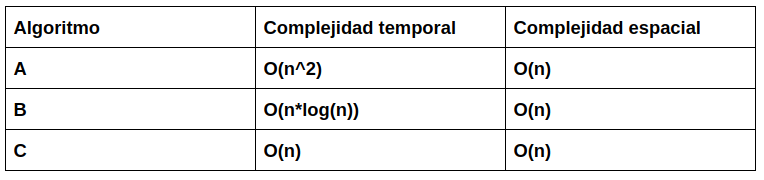
\includegraphics[width=\linewidth]{comparacion.png}
\end{figure}


Como se ve en la tabla, aunque todos tengan la misma complejidad espacial, el Algoritmo C supera a los demás, ya que es óptimo temporalmente.

\newpage
\section{Instalación y ejecución}

El nombre del programa es \textbf{mayoritario}. Para compilar el programa se necesita tener 
instalado \textit{CMake 3.15} o superior. 
Desde la carpeta mayoritario ejecutar los siguientes comandos:

Linux / Windows:

\begin{lstlisting}
    cmake -DCMAKE_BUILD_TYPE=Release .
    make    
\end{lstlisting}


Para ejecutar el programa se debe indicar el tipo de proceso a, b, ó c, el nombre del archivo con el listado de numeros 
que indican el volumen de todas las piezas en un lote.

\begin{lstlisting}
    mayoritario --proceso [a|b|c] --archivo [ruta de archivo]
\end{lstlisting}

Luego ejecutar de la siguiente manera:

\begin{lstlisting}
    ./mayoritario --proceso b --archivo piezas.txt
\end{lstlisting}

Resultado:
\begin{lstlisting}
$ ./mayoritario --proceso b --archivo piezas.txt
El elemento mayoritario es: 110    
\end{lstlisting}



\end{document}